+\documentclass[12pt]{article}
 +
 +\usepackage[table]{xcolor}
 +
 +\usepackage[hidelinks]{hyperref}
 +\usepackage{etoolbox}
 +\usepackage{graphicx}
 +\usepackage{adjustbox}
 +
 +\makeatletter
 +\def\ScaleIfNeeded{%
 +  \ifdim\Gin@nat@width>\linewidth
 +    \linewidth
 +  \else
 +    \Gin@nat@width
 +  \fi
 +}
 +\makeatother
 +
 +% fonts
 +\usepackage[T1]{fontenc}
 +\usepackage[utf8]{inputenc}
 +\usepackage{textgreek}
 +\usepackage[greek,english]{babel}
 +\usepackage{amsmath}
 +
 +% Code highlight and colors
 +\usepackage{listings}
 +\lstset{
 +  numbers=left,
 +  tabsize=1,
 +  basicstyle=\small\ttfamily,
 +  breaklines=true
 +}
 +
 +\usepackage{booktabs, tabularx, longtable}
 +\usepackage{csquotes}
 +\usepackage{authblk}
 +
 +% Geometry block
 +\usepackage[letterpaper]{geometry}
 +\providecommand{\tightlist}{\setlength{\itemsep}{0pt}\setlength{\parskip}{0pt}}
 +
 +\title{How do dispersal effect weed dynamics? Sensitivity analysis of
landscape-scale model to Kernel curves}
 +
 + +\author[1,2]{Willian~Vieira}
 + +\author[1]{Benoit~Ricci}
 + +\author[1]{Nathalie~Colbach}
 + + +\affil[1]{INRA, UMR 1347 Agroécologie, BP 86510, F-21000 Dijon, France}
 + +\affil[2]{Département de Biologie, Université de Sherbrooke, Sherbrooke, Québec,
Canada}
 + +
 +\begin{document}
 +
 +\maketitle
 +
 +\begin{abstract}
 +  \section{Paper idea}\label{paper-idea}

\textbf{Theoretical question} - What is the role of dispersal on weed
dynamics? - Could spatial arrangement of management decisions at a
landscape scale decrease weed spread and persistence in agro-ecosystems?
If so, how can proportion of permanent meadows impact weed spread?

\textbf{Technical question} - Are different ways of dispersal
representation (curves) important to consider?

\textbf{Main results} - the better fit of the 2Dt curve to represent
weed dispersion (this answers the first theoretical question and the
technical one). - And the impact of permanent meadows on the spread of
weed dispersion. Briefly, increasing permanent meadows decreases the
propagation speed of weed seeds (this answers the second theoretical
question)

\textbf{Paper structure}:\\
Based in the above ideas and results, the paper will be structured in
first answering if there is an impact of dispersion representation on
weed dynamics. We will show that there is a significant impact of the
curve but not considerable when compared with land use variation, in
anyways, the 2Dt curve fitted best the data. Next, to answer if land use
variation can change weed dynamics, we will use a case study with
simulations based in the introduction of weed species in non-colonized
landscapes. Here we show that increasing permanent meadows decreases
propagation speed, where the proportion of land use, together with the
type of land use, plays a major role in weed dynamics.
 +\end{abstract}
 +
 +% pandoc-xnos: cleveref fakery
\newcommand{\plusnamesingular}{}
\newcommand{\starnamesingular}{}
\newcommand{\xrefname}[1]{\protect\renewcommand{\plusnamesingular}{#1}}
\newcommand{\Xrefname}[1]{\protect\renewcommand{\starnamesingular}{#1}}
\providecommand{\cref}{\plusnamesingular~\ref}
\providecommand{\Cref}{\starnamesingular~\ref}
\providecommand{\crefformat}[2]{}
\providecommand{\Crefformat}[2]{}

% pandoc-xnos: cleveref formatting
\crefformat{figure}{fig.~#2#1#3}
\Crefformat{figure}{Figure~#2#1#3}
\crefformat{table}{table~#2#1#3}
\Crefformat{table}{Table~#2#1#3}
\crefformat{equation}{eq.~#2#1#3}
\Crefformat{equation}{Equation~#2#1#3}

\section{Introduction}\label{introduction}

\emph{to be done: step 4}

One of the issues in agroecology is to design innovative crop systems
and identify arrangements of natural habitats in the landscape that
allow both to control the abundances of weeds and to preserve their role
in the ecosystem services. It is also important to understand ecological
process of landscape effects on population dynamics.

Discuss the overall theoretical knowledge of plant dispersal with an
emphasis in short-lived plants and weed species.

Try and show the well-known role that dispersal plays in plant dynamics
and what could be true/false for weed communities in a human
environment.

In the above context, DynWeed was created to represent the dynamics of
weed in a landscape scale, which makes necessary take dispersal into
account. However, Modeling the dispersion is difficult because of the
high variability of dispersion distance and the lack of empirical data.
This is the context of the \enquote{technical question}. Discuss the
technical part of dispersal (e.g.~curves) and how it has been modeled.

Here we ask the following questions: (i) what is the role of dispersal
on weed dynamics? (ii) Does dispersal curve really matters at
landscape-action? (iii) Could spatial arrangement of management
decisions at landscape scale decrease weed spread and persistence in
agro-ecosystems? If so, (iv) how can proportion of permanent meadows
impact weed spread? Using a landscape-scale model, our hypothesis is
that different curves to represent the dispersal process will change
dispersal distance and hence the weed dynamics. Furthermore, increasing
the proportion permanent meadows in the agricultural landscape will
reduce the speed of weed spread through the landscape. These will
provide mechanist insights into local weed management and into landscape
spatial arrangement of management decisions, with suggestions to
empirical research and decision makers.

\section{Methods}\label{methods}

\subsection{Population dynamics model}\label{population-dynamics-model}

We used a spatially explicit model of population dynamics for four
different weed species in agricultural landscape (Ricci et al. 2017).
Based in the population dynamics of weed species, the model has five
parameters representing the natural process: the seed germination
\emph{(gr)} and mortality (\emph{sm}) rate, the quantity of seed
produced per plant (\emph{sp}), the plant mortality rate (\emph{pm}) and
the environmental carrying capacity (\emph{K}). Let \emph{P} be the
density of plants at time \emph{t} (\xrefname{eq.}\cref{eq:p}), this
variable increases with viable seeds germinating at rate \emph{(1 -
sm)gr}, and with the number of survival plants \emph{(1 - pm)} times the
seed production (\emph{S}). The density of viable seeds (\emph{S};
\xrefname{eq.}\cref{eq:s}) is a function of either germinated seeds
\emph{(1 - sm)} and the seed bank \emph{(1 - gr)}, plus the proportion
of dispersed seeds from other patches, which is calculated by different
dispersal curves \emph{D} (\Xrefname{Table}\Cref{tbl:eq}).

\begin{equation} P_{t,x,y} = min\{K,(1 - sm_{t,x,y})gr\times(1 - pm_{t,x,y})S_{t-1,x,y}\} \label{eq:p}\end{equation}

\begin{equation} S_{t,x,y} = (1 - sm_{t,x,y})\times(1 - gr_{t,x,y})S_{t-1,x,y} + \iint\limits_{(x',y')} (P_{t,x',y'}sp_{t,x',y'})D(x - x', y - y') \label{eq:s}\end{equation}

\subsection{Dispersal curves and
parameterization}\label{dispersal-curves-and-parameterization}

We tested four kernel curves to represent the process of weed dispersion
(\Xrefname{Table}\Cref{tbl:eq}).

\begin{longtable}[]{@{}lrcc@{}}
\caption{Kernel curves to calculate the probability of seed dispersal,
the parameter assumptions and the distribution form.
\label{tbl:eq}}\tabularnewline
\toprule
\begin{minipage}[b]{0.17\columnwidth}\raggedright\strut
Curve\strut
\end{minipage} & \begin{minipage}[b]{0.15\columnwidth}\raggedleft\strut
Equation\strut
\end{minipage} & \begin{minipage}[b]{0.16\columnwidth}\centering\strut
Parameters\strut
\end{minipage} & \begin{minipage}[b]{0.18\columnwidth}\centering\strut
Distribution\strut
\end{minipage}\tabularnewline
\midrule
\endfirsthead
\toprule
\begin{minipage}[b]{0.17\columnwidth}\raggedright\strut
Curve\strut
\end{minipage} & \begin{minipage}[b]{0.15\columnwidth}\raggedleft\strut
Equation\strut
\end{minipage} & \begin{minipage}[b]{0.16\columnwidth}\centering\strut
Parameters\strut
\end{minipage} & \begin{minipage}[b]{0.18\columnwidth}\centering\strut
Distribution\strut
\end{minipage}\tabularnewline
\midrule
\endhead
\begin{minipage}[t]{0.17\columnwidth}\raggedright\strut
Gausian\strut
\end{minipage} & \begin{minipage}[t]{0.15\columnwidth}\raggedleft\strut
\[ f(x) = \frac{1}{\theta\sqrt{2\pi}} e^{\frac{-x^2}{\theta y^2}} \]\strut
\end{minipage} & \begin{minipage}[t]{0.16\columnwidth}\centering\strut
\(\theta\) \textgreater{} 0\strut
\end{minipage} & \begin{minipage}[t]{0.18\columnwidth}\centering\strut
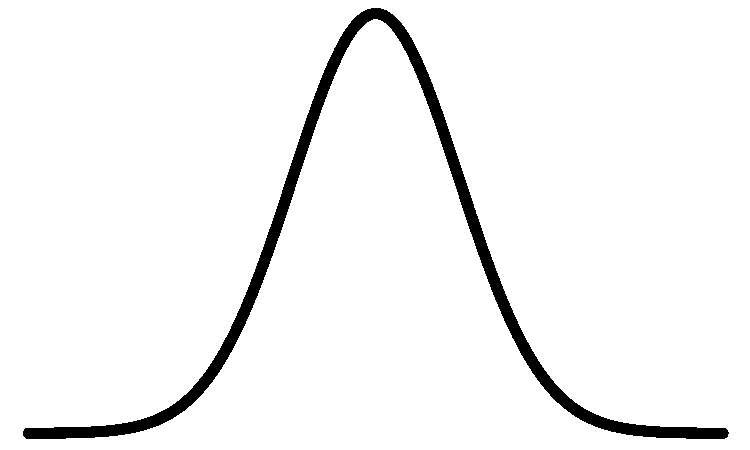
\includegraphics[width=0.65000\textwidth]{figure/gaussian.pdf}\strut
\end{minipage}\tabularnewline
\begin{minipage}[t]{0.17\columnwidth}\raggedright\strut
Weibull\strut
\end{minipage} & \begin{minipage}[t]{0.15\columnwidth}\raggedleft\strut
\[ f(x) = \frac{\epsilon - 1}{\epsilon\phi^\epsilon} \epsilon x^{\epsilon - 1} e^{\frac{\epsilon - 1}{\epsilon\phi^\epsilon}x^\epsilon} \]\strut
\end{minipage} & \begin{minipage}[t]{0.16\columnwidth}\centering\strut
\(\epsilon\) \textgreater{} 1 \(\phi\) \textgreater{} 0\strut
\end{minipage} & \begin{minipage}[t]{0.18\columnwidth}\centering\strut
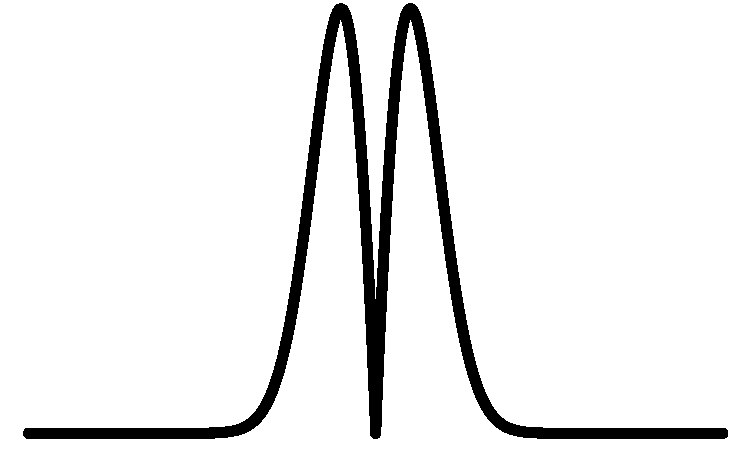
\includegraphics[width=0.65000\textwidth]{figure/weibull.pdf}\strut
\end{minipage}\tabularnewline
\begin{minipage}[t]{0.17\columnwidth}\raggedright\strut
Exponential\strut
\end{minipage} & \begin{minipage}[t]{0.15\columnwidth}\raggedleft\strut
\[ f(x) = \frac{1}{2\pi\lambda^2} e^{\frac{-x}{y}} \]\strut
\end{minipage} & \begin{minipage}[t]{0.16\columnwidth}\centering\strut
\(\lambda\) \textgreater{} 0\strut
\end{minipage} & \begin{minipage}[t]{0.18\columnwidth}\centering\strut
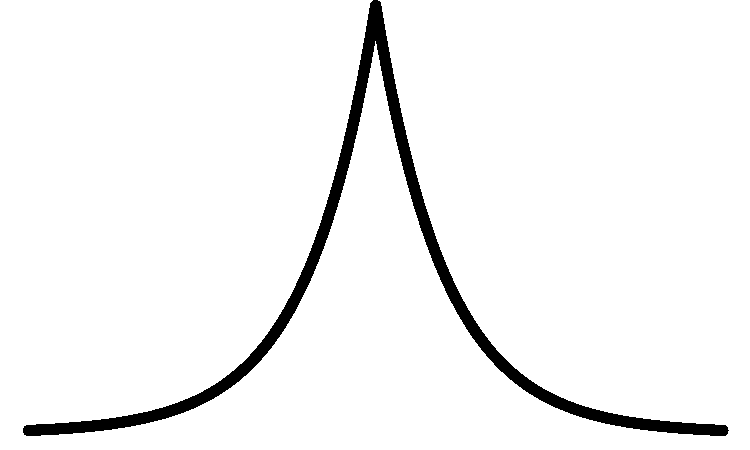
\includegraphics[width=0.65000\textwidth]{figure/exponential.pdf}\strut
\end{minipage}\tabularnewline
\begin{minipage}[t]{0.17\columnwidth}\raggedright\strut
2Dt\strut
\end{minipage} & \begin{minipage}[t]{0.15\columnwidth}\raggedleft\strut
\[ f(x) = \frac{\beta - 1}{\alpha^2 \pi} 1 + (\frac{x^2}{y^2})^{-\beta} \]\strut
\end{minipage} & \begin{minipage}[t]{0.16\columnwidth}\centering\strut
\(\alpha\) \textgreater{} 0 \(\beta\) \textgreater{} 1\strut
\end{minipage} & \begin{minipage}[t]{0.18\columnwidth}\centering\strut
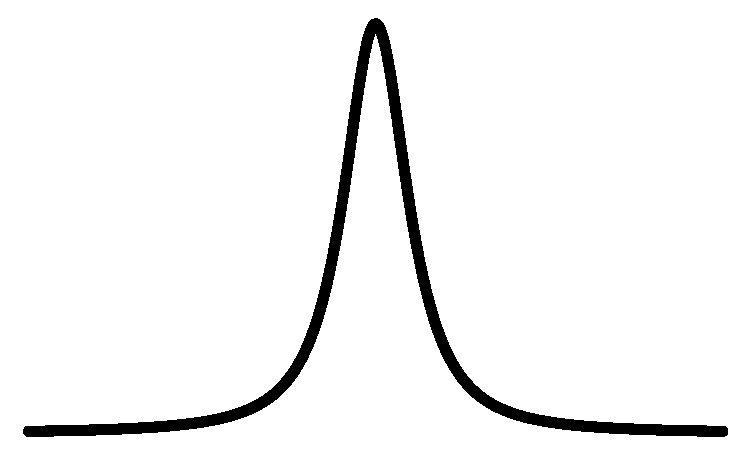
\includegraphics[width=0.65000\textwidth]{figure/2dt.pdf}\strut
\end{minipage}\tabularnewline
\bottomrule
\end{longtable}

Show here how I chose each value of parameter and where this values come
from (curve fitted based in Thomson et al. (2011))

\subsection{Dispersal calculation}\label{dispersal-calculation}

The seed spread calculation was based\ldots{}

\subsection{Simulation plan}\label{simulation-plan}

Explain the variation of each simulation.

\subsection{Statistics analysis}\label{statistics-analysis}

Test (Gaba et al. 2010)

\section{Results}\label{results}

\emph{to be done: step 2}

The speed of seed spread over time shows a median of 262.2
meters.year\^{}\{-1\} (from 62.7 to 402.9) for all simulations. This
speed is mostly influenced by land use (ω2mean = 15.4\%) and by the
interaction of curve and proportion of land use (ω2mean = 10\%; table
1). Both the proportion of land use and the curve alone has a moderate
effect on the speed of spread (5.8\% and 5.3\%, respectively). Among the
landscape with a unique land use, the permanent meadows presented the
slowest median dissemination speed (80 metersyear-1) compared with
conventional (266.6) and organic (279). Increasing the proportion of
permanent meadows to 50\% in the landscape significantly decreased the
dissemination speed, but there was no difference when increased to 3\%
(Figure 1). The significantly but weak effect of the dispersion curve on
dissemination speed (ω2mean = 5.3\%), shows a general higher median
dissemination speed for the 2Dt curve (282.3 metersyear-1) compared with
Exponential (268.8), Gaussian (265.3) and Weibull (265.3; Figure 1).

\section{Discussion}\label{discussion}

\emph{to be done: step 3}

\section*{References}\label{references}
\addcontentsline{toc}{section}{References}

\hypertarget{refs}{}
\hypertarget{ref-Gaba2010}{}
\textbf{Gaba et al.} (2010). Weed species richness in winter wheat
increases with landscape heterogeneity. \emph{Agriculture, Ecosystems
and Environment.} Elsevier B.V. 138:318--23.

\hypertarget{ref-Ricci2017}{}
\textbf{Ricci et al.} (2017). How much can a large scale planning reduce
local weed infestations ? A landscape-scale modelling approach.
\emph{Ecological Modelling.}:Submitted.

\hypertarget{ref-Thomson2011}{}
\textbf{Thomson et al.} (2011). Seed dispersal distance is more strongly
correlated with plant height than with seed mass. \emph{Journal of
Ecology.} 99:1299--307.
 +
 +\end{document}
